\chapter{Artificial neural networks}
\label{chap:neuralNetworks}

\lettrine{A}{rtificial} neural networks (ANN) are a set of algorithms inspired by biological neural networks. They are the core components of deep learning \cite{goodfellow_deep_2016}, which itself can be defined as a part of machine learning. Machine learning refers to the capabilities of certain systems to learn how to perform a specific task, having been provided with an appropriate data for training. At the time of this thesis writing, in 2021, more and more applications have proven how much deep learning has improved the performance of machines in many various tasks, \emph{e.g.}, in image recognition \cite{he_deep_2016}, machine translation \cite{vaswani_attention_2017}, speech recognition \cite{hinton_deep_2012}, sound source separation \cite{hennequin_spleeter_2020}, board game playing \cite{silver_mastering_2017}, protein structure prediction \cite{jumper_highly_2021}, or music generation \cite{hadjeres_deepbach_2017}. While it has been shown that any task can be learned with a three-layer neural network \cite{hornik_multilayer_1989}, neural systems generally consist of many layers connected together, resulting in deep neural architectures, hence the term \textit{deep learning}. 

Many neural network architectures have been proposed in the past, and many of them were initially designed for a specific task, \emph{e.g.}, convolutional neural networks (CNN) for image recognition \cite{lecun_backpropagation_1989} or attention mechanism for machine translation \cite{he_deep_2016}. Due to their success, it is common to encounter adaptations of these architectures to address problems other than the original ones: for example, CNNs have been widely used for audio related tasks \cite{purwins_deep_2019}, while attention-based neural networks are commonly applied for computer vision \cite{dosovitskiy_image_2021}.

In this chapter, we provide a short overview of deep learning, and more precisely of different types of neural networks which were used throughout this thesis. Although the exploitation of artificial neural networks (ANN) is relatively new in the SSL literature (see Section~\ref{sec:SSLliterature}), deep learning is widely established in the audio research community, so this section is written assuming that the reader has some basic background on ANNs. We describe the different neural network architectures and mechanisms we exploited in this thesis. We assume this short introduction will be sufficient to help the reader to easily follow the experiments described in the next chapters. If needed, more in-depth description of deep learning can be found in \cite{goodfellow_deep_2016}. 

This chapter is organized as follows. Section~\ref{sec:mlp} introduces the basics of ANNs and the multilayer perceptron. Section~\ref{sec:cnn} explains the inner workings of a CNN, while Section~\ref{ss:recurrentNeuralNetworks} deals with recurrent neural networks (RNNs). Section~\ref{ss:residualNetworks} proposes a quick summary of residual connections. Finally, Section~\ref{sec:attentionMechanisms} describes the attention mechanism.

%-----------------------------------------------
%  MULTILAYER PERCEPTRON
%-----------------------------------------------
\section{Multilayer perceptron and backpropagation algorithm}
\label{sec:mlp}

\subsection{Multilayer perceptron or feedforward neural network}

A \textit{multilayer perceptron} (MLP) is a particular kind of artificial neural network in which all the connections are made forward, hence its name. In this section, we describe how an MLP can approximate a function using layers of artificial neurons and activation functions. We also explain how such a neural network can be trained with the backpropagation algorithm, with a review of loss functions and output units used throughout this thesis.

\subsubsection{Artificial neurons}

The fundations of artificial neural networks have been proposed as early as 1943 when McCulloch and Pitts \cite{mcculloch_logicial_1943} established a computational model of biological neurons. An artificial neuron is the building block of an ANN, and is composed of two stages :
\begin{itemize}
    \item A linear combination of its entries, using a set of weights specific to this neuron, as in \eqref{eq:artificialNeuron}
    \item The addition of a bias $b$
    \item An activation function $\sigma$ applied after the linear combination
\end{itemize}
\begin{equation}
\label{eq:artificialNeuron}
    y = \sigma \Big( \sum_{i=1}^{I} \theta_i x_i + b \Big),
\end{equation}
where $\{\theta_i\}_i$ and $b$ form the parameters of the neuron, $x_i$ are the entries of the input $\mathbf{x}$ and $y$ is the (scalar) output. We often set $b=\theta_0$ and append $1$ to the input vector so that $\{\theta_i\}_i$ is the entire set of weights.

Generally, multiple neurons are assembled to form a \textit{layer}, in which all the neurons are input with the same vector $\mathbf{x}$, thus each neuron of the same layer contains the same number of weights. An \textit{artificial neural network} is then defined to be a succession of $H$ layers of artificial neurons ($H$ is known as the \textit{depth} of the network), each layer being fed with the vector formed by the output of all neurons from the previous layer. If the layer $h$ is composed of $I_h$ neurons with input $\mathbf{x}^{h-1}$ (with $I_{h-1}$ components), then the entries of the output vector $\mathbf{x}^h$ are:
\begin{equation}
\label{eq:layerOutput}
    x_j^h = \sigma \bigg( \sum_{i=1}^{I_{h-1}} \theta_{j,i}^h x_i^{h-1} + b_j^h \bigg),
\end{equation}
for all $j \in \{1, ..., I_h\}$. This type of layer is called a \textit{fully-connected} layer or a \textit{feedforward} (FF) layer. The layer at $h=1$ is known as the \textit{input} layer, which directly receives the input features to its entries, and the last layer at $h=H$ is known as the \textit{output} layer. We generally name the output vector $\mathbf{y}$. The other layers are termed \textit{hidden} layers. 

We can rewrite \eqref{eq:layerOutput} in a more compact manner as:
\begin{equation}
\label{eq:layerOutputVectorized}
    \mathbf{x}^h = \sigma(\mathbf{b}^h + \mathbf{W}^h \mathbf{x}^{h-1}),
\end{equation}
where $\mathbf{b}^h$ is the \textit{bias} vector of layer $h$ and $\mathbf{W}^h$ is the weight matrix in $\mathbb{R}^{I_h \times I_{h-1}}$. This computation is known as a \textit{forward pass}.

The universal approximation theorem \cite{hornik_multilayer_1989} states that a MLP with two layers and a non-polynomial activation function at the first layer can approximate any function $f$ with an arbitrary accuracy.

\subsubsection{Activation functions}

There is a number of non-polynomial activation functions commonly used in the DL literature, as well as in this thesis. Linear activation functions are mostly used at the output layer, when the network is used in regression mode (see Section~\ref{ss:outputScheme}).

The \textit{rectified linear unit} (ReLU) is one of the most used activation function:
\begin{equation}
    \sigma(x) = max(0,x), \quad \forall x \in \mathbb{R}.
\end{equation}
This function has the advantage to preserving some of the properties that make linear models generalize well \cite{goodfellow_deep_2016}. 

The \textit{sigmoid} function is defined by:
\begin{equation}
    \sigma(x) = \frac{1}{1+e^{-x}}, \quad \forall x \in \mathbb{R}.
\end{equation}
Its values are always in $[0,1]$, and it converts large negative values to $0$ and large positive values to $1$. It is often used as an output activation function with its output value seen as a probability, which is particularly suitable for binary classification problems. Sometimes, the \textit{hard sigmoid} is preferred for its sharper contour:
\begin{equation}
    \sigma(x) = max\Big(0,min\big(1,\frac{x+1}{2}\big)\Big), \quad \forall x \in \mathbb{R}.
\end{equation}
The \textit{hyperbolic tangent (tanh)} function is defined by:
\begin{equation}
    \sigma(x) = \frac{e^{2x}-1}{e^{2x}+1}, \quad \forall x \in \mathbb{R}.
\end{equation}
The shape of tanh ressembles the shape of the sigmoid but it takes values within $[-1,1]$. Finally, the \textit{softmax} function is a generalization of the sigmoid function and produces a set of values within $[0,1]$:
\begin{equation}
    \sigma(y_i) = \frac{e^{x_i}}{\sum_{i=0}^{I} e^{x_i}},
\end{equation}
where $x_i$ and $y_i$ are the components of vectors $\mathbf{x}$ and $\mathbf{y}$, respectively. This function ensures that $\mathbf{y}$ can be seen as a probability distribution since its entries sum to $1$, which is particularly suitable for multi-class classification problems.


\subsection{The backpropagation algorithm}
\label{sec:backpropagationAlgorithm}

During the training stage, a neural network can adjust its weights with an algorithm called \textit{backpropagation} -- other algorithms exist - each time it is fed with a training example. To do that, the neural network performs a forward pass with training example $\mathbf{x}$, which gives an output value $\hat{\mathbf{y}}$. After choosing a \textit{loss} (or \textit{cost}) function $\mathcal{L}$, the knowledge of the target value $\mathbf{y}$ (which is known as the \textit{label} or \textit{ground-truth} of data $\mathbf{x}$) leads to the computation of the error made by the neural network for input $\mathbf{x}$, $\mathcal{L}(\mathbf{y},\hat{\mathbf{y}})$. The backpropagation algorithm uses this value $\mathcal{L}(\mathbf{y},\hat{\mathbf{y}})$ to adjust the weights of the neurons with a gradient descent. If at iteration $t$ of the backpropagation algorithm the weights are $\mathbf{w}^t$ (we drop the index $h$ for better visualization), the new value $\mathbf{w}^{t+1}$ at iteration $t+1$ is:
\begin{equation}
    \mathbf{w}^{t+1} = \mathbf{w}^{t} - \eta \frac{\partial \mathcal{L}(\mathbf{y}, \hat{\mathbf{y}})}{\partial \mathbf{w}^{t}},
\end{equation}
where $\eta$ is known as the \textit{learning rate}. This operation is done for all weights and for all training examples, by the means of training batches (composed of a certain numbers of these training examples), until some convergence criterion is met. In practice, the neural network is fed with the whole training set (each training pass using the whole training set is called an \textit{epoch}) for a certain number of times.

\subsubsection{Loss functions}

The choice for the loss function $\mathcal{L}$ depends on the output strategy employed to learn the considered task. The idea is to opt for a function that penalizes the difference between the ground-truth $\mathbf{y}$ and the estimated value $\hat{\mathbf{y}}$ with a sufficiently large value so that the change in weights due to gradient descent is significant. Moreover, loss functions are generally applied ``simultaneously'' on subsets of training examples called \textit{training batches}. In the following, we define the loss functions only for one training example, while for training batches the loss is obtained by summing the losses of all batch examples. Throughout this thesis, several loss functions were exploited:
\begin{itemize}
    \item Mean squared error (MSE) : $\mathcal{L}(\mathbf{y},\hat{\mathbf{y}}) =  \frac{1}{I} \sum_i^I (y_i - \hat{y}_i)^2$. When computing the loss for a training batch, the sum of all losses is divided by the number of examples in the batch, hence the term \textit{mean}. It is often used with a regression paradigm.
    
    \item Categorical cross-entropy : $\mathcal{L}(\mathbf{y},\hat{\mathbf{y}}) = - \sum_{i=1}^I y_i log(\hat{y}_i)$. This cross-entropy can be used for a classification problem, for which $\mathbf{y}$ is a one-hot vector (all entries are set to 0 except the one corresponding to the class which is set to 1). The softmax activation function suits well to this loss function.
    
    \item Binary cross-entropy : $\mathcal{L}(y,\hat{y}) = - y log(\hat{y}) + (1-y) log(\hat{y})$, which a particular case of the categorical cross-entropy when $I=1$, \emph{i.e.} the output is a scalar. It is generally used when $\mathbf{y}$ has a binary value ($0$ or $1$) and in conjonction with the sigmoid function which bounds the values of $\hat{\mathbf{y}}$ in $[0,1]$. If $\mathbf{y}$ and $\hat{\mathbf{y}}$ are vectors with binary values, the loss is obtained by summing the binary cross-entropy for each vector entry.
    
\end{itemize}

\subsection{Avoiding overfitting}

A major problem in neural networks is that the model can lack generalization when it is applied on data unseen during the training stage. This phenomenon is called overfitting, and part of deep learning research has been dedicated to avoid it and make the neural network to generalize better on unseen data. One strategy to control the learning of a neural network is to make use of a \textit{validation} dataset, which does not contain common data with the training dataset. During the training phase, the performance of the neural network is evaluated on the validation dataset (hence unseen data), and the training is stopped when the performance starts decreasing, meaning that the model starts overfitting on the training data. This monitoring method is known as \textit{early stopping}.

Another common regularization method is \textit{dropout} \cite{srivastava_dropout_2014}. It relies on bypassing random neurons (except for those in the output layer) based on a user-adjustable probability so that the output of these neurons are fixed to zero. This enforces the neural network not to overuse some specific neurons, and consequently prevents overfitting. This technique is employed only during training. Finally, batch normalization is a technique which can make a neural network more stable by rescaling and recentering the data in-between layers.

These methods were regularly used all along the experiments in this thesis.

%-----------------------------------------------
%  CONVOLUTIONAL NEURAL NETWORKS
%-----------------------------------------------
\section{Convolutional neural networks}
\label{sec:cnn}

Convolutional neural networks (CNN) are neural networks including convolutional layers which are specifically well-designed for processing data presented as a grid, for instance images represented by pixels. It has been pioneered in the end of the 1980s by LeCun et al. \cite{lecun_backpropagation_1989} to recognize handwritten digits in images. Since then, other new ideas around convolutional layers have been proposed in the literature. This section aims to provide a quick overview of CNNs, since they were used in our experiments.

\subsection{Convolutional layers}

As its name indicates, a convolutional layer applies convolutions on its input to produce an output, using a series of convolution kernels (or filters) $k$ which contain the learnable weights. In the 1D discrete domain (\emph{e.g.}, discrete time), this convolution is expressed by:
\begin{equation}
    y(n) = (x * k)(n) = \sum_i x(n-i)k(i),
\end{equation}
where $x$ and $y$ are the input and output, respectively, and $n$ is the discrete sample index. In practice, the kernel $k$ is a vector with a fixed size, so the sum is in a finite corresponding range. 

In the 2D domain, the convolution is applied in both dimensions:
\begin{equation}
    y(m,n) = (x * k)(m,n) = \sum_i \sum_j x(m-i,m-j) k(m,n).
\end{equation}
In this case, the kernel is a 2D matrix, and the same consideration applies regarding the range of the summation. Fig.~\ref{fig:2DconvolutionKernel} illustrates how a single 2D kernel of size $3 \times 3$ would be applied for each pixel of an input image.

\begin{figure}[t]
    \begin{center}
    \includegraphics[width=1.\linewidth]{Images/chap3/2DConvolutionKernel.png}
    \captionof{figure}[2D convolution operation with a $3 \times 3$ kernel]{2D convolution operation with a $3 \times 3$ kernel. Each $3 \times 3$ region on the image is multiplied with the kernel (right matrix), which is a 2D convolution operation, resulting in a scalar value associated to the region in the output. Zero-padding can optionally be used for regions on the edges. Note that the illustrated kernel is an example of how we can detect vertical contours with convolutions.}
    \label{fig:2DconvolutionKernel}
    \end{center}
\end{figure}

This convolution operation has also been extended to higher dimension, but this will be not used in this thesis. Zero-padding, \emph{i.e.}, automatic completion of input image edges with zeros, can be used  so that the output dimension is exactly the same as the input dimension. In contrast, one can use a \textit{stride}, \emph{i.e.}, a shift of the kernel operator in between two successive convolutions, greater than one so as to limit the size of the output and somehow ``compress'' the data representation, at the price of lower resolution.

During the training phase, the kernel matrix is learnt so that it provides the most meaningful convolution operation for the neural network to perform a task. In a convolutional layer, a bank of (possibly many) different  kernels are generally instantiated, so that each one can perform a specific operation, leading to different higher-level outputs, which are commonly called \textit{feature maps}. These outputs are then stacked, as illustrated in Fig.~\ref{fig:stackedConvolutionKernels}, and can become the input for another convolutional layer. 

\begin{figure}[t]
    \begin{center}
    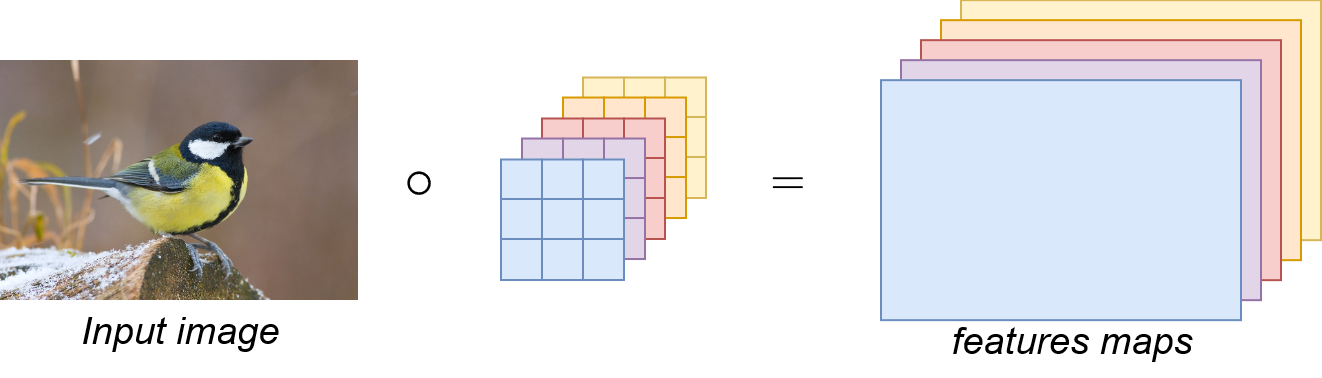
\includegraphics[width=1.\linewidth]{Images/chap3/stackedConvolutionKernels.png}
    \captionof{figure}[Application of multiple convolution kernels on a input image]{Application of multiple convolution kernels on a input image. Each kernel has its own set of learnable weights, and results in specific outputs, which are stacked in what is called feature maps.}
    \label{fig:stackedConvolutionKernels}
    \end{center}
\end{figure}

One major advantage of convolutional layers is that the operations are translation equivariant \cite{bronstein_geometric_2021}. In that way, each kernel can be learnt to highlight specific contours in the input feature, which is why several kernels are assembled in each convolutional layer. The obtained feature maps provide a somehow higher-level representation of the input signal, and stacking several convolutional layers one after another is often employed to perform \textit{feature extractions} in practice.

\subsection{Dilated convolutions}

A generalization of the convolution kernels presented above has been proposed in \cite{yu_multi-scale_2016}, under the name \textit{dilated convolution}. The idea is to apply the kernel on a downsampled version of the data, so that the convolution operation span is increased while keeping the same amount of learnable weights. This dilated convolution can be expressed by \cite{yu_multi-scale_2016}:
\begin{equation}
    (x * k)(n) = \sum_{i} x(n-li)k(i),
\end{equation}
where $l$ is the \textit{dilation factor}. For $l=1$, this operation is equivalent to the classical convolution. The idea can be extended to higher dimensions. Fig.~\ref{fig:dilatedConvolutions} illustrates how these dilated convolutions operate on input data, showing how it increases the convolution operation span. Dilated convolutions are also called \textit{atrous} convolutions, since we can see them as classical kernels with zeros inserted in between the actual weights.

\begin{figure}[t]
    \begin{center}
    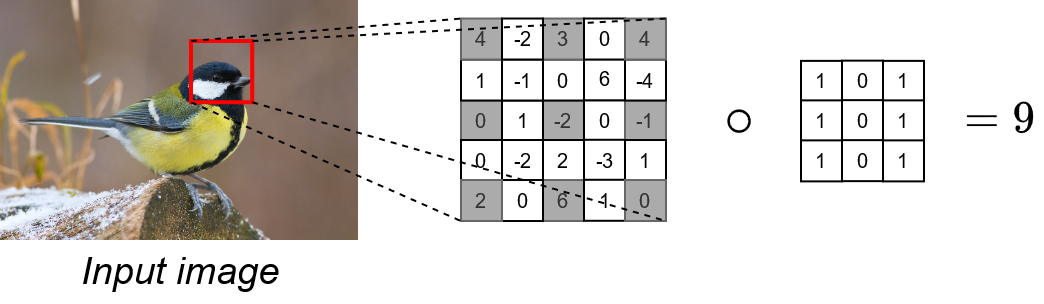
\includegraphics[width=1.\linewidth]{Images/chap3/dilatedConvolutions.png}
    \captionof{figure}[Visualization of dilated convolutions]{Visualization of dilated convolutions with a dilation factor $l=2$.}
    \label{fig:dilatedConvolutions}
    \end{center}
\end{figure}

\subsection{Pooling operation}

Pooling layers are also very common when using convolutional layers in neural networks. The goal of these layers is to downsample the data to reduce its dimensionality. The pooling size indicates the region shape in which only one value is extracted. If max-pooling is used, the highest value is kept, while if average pooling is used, the extracted value is the mean of all values in the corresponding region. As with convolutional layers, one can opt for a stride value, \emph{i.e.}, a shift that will skip data when applying the pooling operation. Fig.~\ref{fig:maxPooling} illustrates the max-pooling operation with a pooling size of $2 \times 2$ and a stride of $2$.

\begin{figure}[t]
    \begin{center}
    \includegraphics[width=0.6\linewidth]{Images/chap3/maxPooling.png}
    \captionof{figure}[Max-pooling operation]{Max-pooling operation. The operation is downsampling the data by keeping only the highest value of a considered region., In this example, the pooling size is $2 \times 2$ and the stride is $2$.}
    \label{fig:maxPooling}
    \end{center}
\end{figure}

%-----------------------------------------------
%   RECURRENT NEURAL NETWORKS
%-----------------------------------------------
\section{Recurrent neural networks}
\label{ss:recurrentNeuralNetworks}

Recurrent neural networks (RNN) are a family of neural networks that are suitable for processing sequential data, in which the ordering of successive data vectors bears importance. With MLPs or CNNs, data are processed one layer after another, without memorizing the operations within the network. The idea behind RNNs is to keep in memory some values (called \textit{states}) that contain a summary of past data information and which are used for further computation of the present output vector.

\subsection{Basic recurrent neural networks}

We consider a sequence of data vectors $\mathbf{x}^t$ where $t \in \{1,..., T\}$ is analog to a time index (although it could be any sequential index). In a basic recurrent layer, at each timestep $t$, a hidden vector $\mathbf{h}^t$ is considered in addition to the input vector $\mathbf{x}^t$. First, the hidden vector $\mathbf{h}^t$ is computed from the previous hidden vector $\mathbf{h}^{t-1}$ and the current input vector $\mathbf{x}^t$:
\begin{equation}
    \mathbf{h}^t = \sigma_h(\mathbf{W}_h \mathbf{h}^{t-1} + \mathbf{W}_x \mathbf{x}^t + \mathbf{b}),
\end{equation}
where $\mathbf{W}_h$ and $\mathbf{W}_x$ are weight matrices and $\mathbf{b}$ is the bias weight vector. Then, the output vector is computed as :
\begin{equation}
    \mathbf{y}^t = \sigma_y(\mathbf{W}_y \mathbf{h}^t),
\end{equation}
with $\mathbf{W}_y$ being the layer output weight matrix. Note that the activation functions $\sigma_h$ and $\sigma_y$ are not necessarily the same.
Fig.~\ref{fig:basicRecurrentLayer} illustrates how a basic recurrent layer processes data.

\begin{figure}[t]
    \begin{center}
    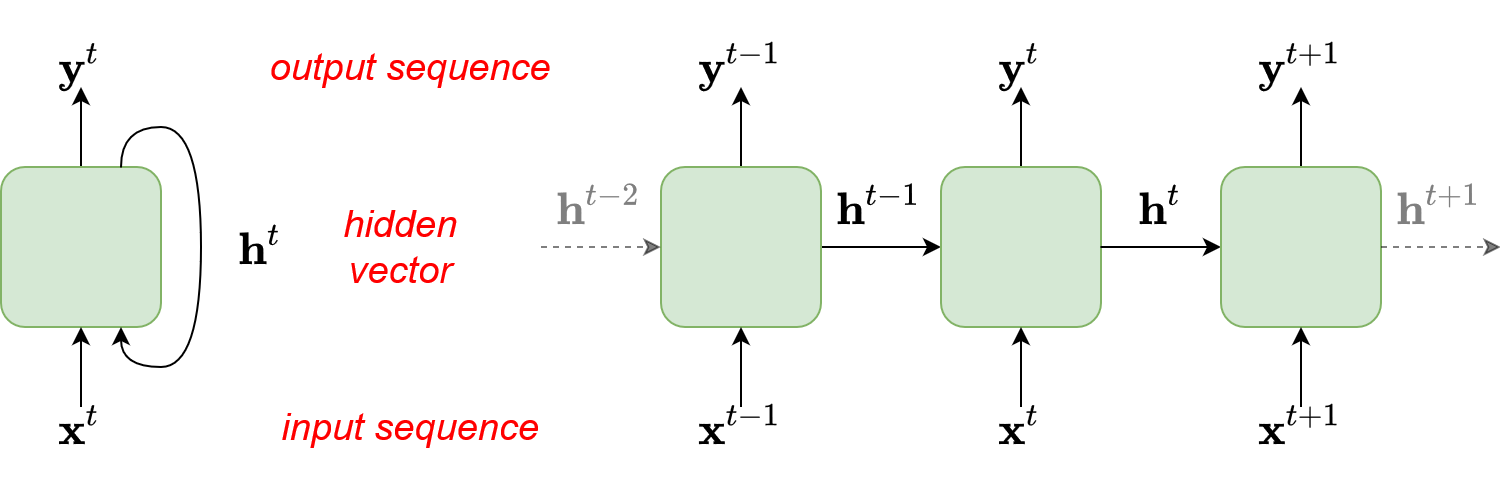
\includegraphics[width=1.\linewidth]{Images/chap3/basicRecurrentLayer.png}
    \captionof{figure}[Compact and unrolled visualization of a basic recurrent layer]{Compact (left) and unrolled (right) visualization of a basic recurrent layer.}
    \label{fig:basicRecurrentLayer}
    \end{center}
\end{figure}

Note that recurrent layers are often employed besides convolutional layers to form a convolutional recurrent neural network (CRNN).

\subsection{Backpropagation through time and vanishing gradient}

With the way a recurrent neural network is defined, one has to turn the usual backpropagation algorithm presented in Section~\ref{sec:backpropagationAlgorithm} into what is referred as backpropagation through time (BPTT). Without giving all details which can be found, \emph{e.g.}, in \cite{goodfellow_deep_2016}, the idea is to unfold the recurrent layer and consider the weights to be shared by each step. BPTT first relies on computing the loss for all timesteps of all sequences in the training batch. Then the gradient of the total loss for a specific weight is obtained as the sum of the gradients for each timestep. However the gradients for timesteps $t>0$ depends on the gradients for previous timesteps $t'<t$, so one needs to iterate backwards through time in order to compute all the gradients (hence the name BPTT).

One well-known limitation of this algorithm is the so-called \textit{vanishing gradient problem}. As the gradients are computed in an iterative way, some gradient values can become very small thus preventing the weight from changing its value. The more iterations are considered the more pronounced is this phenomenon.

\subsection{Long short-term memory}
\label{ss:lstm}

\begin{figure}[t]
    \begin{center}
    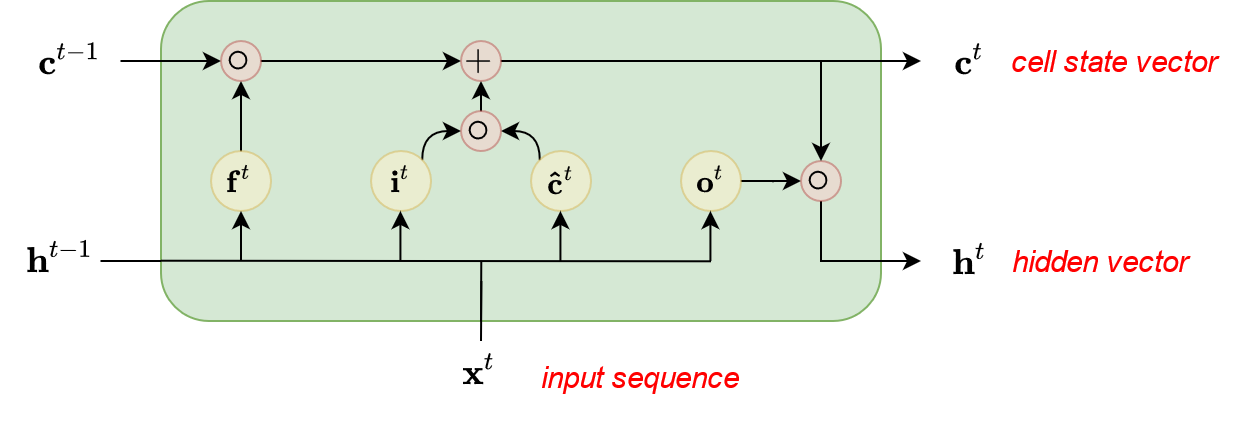
\includegraphics[width=1.\linewidth]{Images/chap3/lstm.png}
    \captionof{figure}[Long short-term memory cell mechanism]{Long short-term memory cell mechanism. In this diagram the activation functions are not shown for the sake of clarity. The gates are displayed in yellow whereas the operations are in red, with $\circ$ denoting the Hadamard (element-wise) product.}
    \label{fig:lstm}
    \end{center}
\end{figure}

The long short-term memory (LSTM) is a recurrent architecture proposed in 1997 by Hochreiter and Schmidhuber \cite{hochreiter_long_1997}, as a means to cope with the vanishing gradient problem, by keeping the error in the LSTM cells. Fig.~\ref{fig:lstm} illustrates the mechanism behind an LSTM cell. In addition to the input vector $\mathbf{x}^t$ and the hidden vector $\mathbf{h}^t$, this model introduces new vectors which are used as \textit{gates} to control the flow of information inside the LSTM cell. The first four vectors, which are all computed in a similar way with their own weights, are:
\begin{itemize}
    \item a forget gate vector $\mathbf{f}^t$ obtained by:
    \begin{equation}
        \mathbf{f}^t = \sigma_s(\mathbf{W}_{f,x} \mathbf{x}^t + \mathbf{W}_{f,h} \mathbf{h}^{t-1} + \mathbf{b}_f),
    \end{equation}
    
    \item an input gate vector $\mathbf{i}^t$ computed with:
    \begin{equation}
        \mathbf{i}^t = \sigma_s(\mathbf{W}_{i,x} \mathbf{x}^t + \mathbf{W}_{i,h} \mathbf{h}^{t-1} + \mathbf{b}_i),
    \end{equation}
    
    \item an output gate vector $\mathbf{o}^t$ expressed by:
    \begin{equation}
        \mathbf{o}^t = \sigma_s(\mathbf{W}_{o,x} \mathbf{x}^t + \mathbf{W}_{o,h} \mathbf{h}^{t-1} + \mathbf{b}_o),
    \end{equation}
    
    \item a cell input activation vector $\mathbf{\hat{c}}^t$ calculated from
    \begin{equation}
        \mathbf{\hat{c}}^t = \sigma_h(\mathbf{W}_{c,x} \mathbf{x}^t + \mathbf{W}_{c,h} \mathbf{h}^{t-1} + \mathbf{b}_c),
    \end{equation}
\end{itemize}
where $\sigma_s$ and $\sigma_h$ are the sigmoid and hyperbolic tangent activation functions, respectively. 

Using the $\mathbf{x}^t$, $\mathbf{i}^t$, $\mathbf{f}^t$ and $\mathbf{\hat{c}}^t$, the cell state vector $\mathbf{c}^t$ (acting like a memory cell), can be obtained by:
\begin{equation}
    \mathbf{c}^t = \mathbf{f} \circ \mathbf{c}^{t-1} + \mathbf{i}^t \circ \mathbf{\hat{c}}^t,
\end{equation}
where $\circ$ denotes the element-wise product.
Finally, the hidden vector $\mathbf{h}_t$ is computed with:
\begin{equation}
    \mathbf{h}_t = \mathbf{o}^t \circ \sigma_h(\mathbf{c}^t).
\end{equation}
In an LSTM cell, the hidden vector $\mathbf{h}^t$ actually acts as the output vector at each timestep $t$.\footnote{Although this seems to contrast with the definition of an RNN, it is actually the way the LSTMs are implemented in most deep learning frameworks such as \textit{Tensorflow} or \textit{PyTorch}.}

\subsection{Gated recurrent units}

\begin{figure}[t]
    \begin{center}
    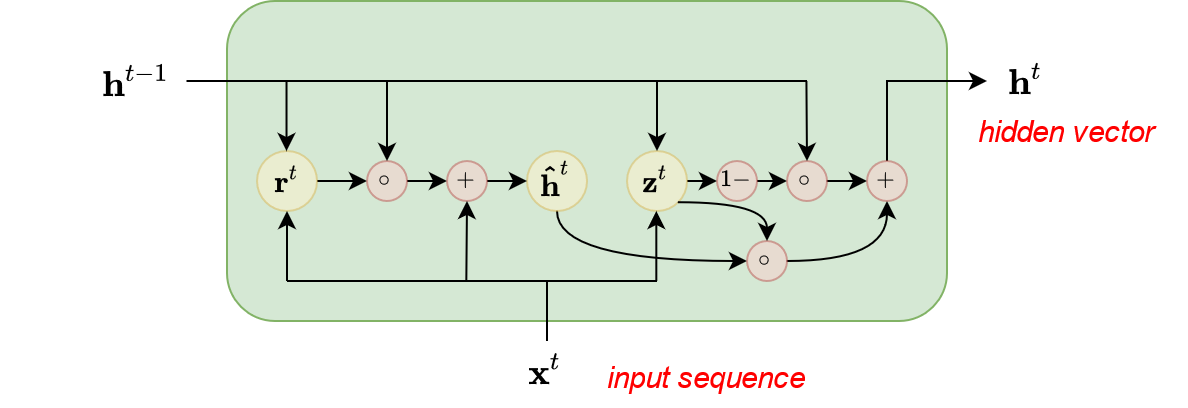
\includegraphics[width=0.9\linewidth]{Images/chap3/gru.png}
    \captionof{figure}[Gated recurrent unit mechanism]{Gated recurrent unit mechanism.}
    \label{fig:gru}
    \end{center}
\end{figure}

In the same vein as LSTMs, gated recurrent units (GRU) \cite{cho_learning_2014} have an internal mechanism which can circumvent the vanishing gradient problem as the error remains in the GRU cells. A GRU is composed of two gate vectors, as illustrated in Fig.~\ref{fig:gru}:
\begin{itemize}
    \item an update gate vector $\mathbf{z}^t$ obtained by:
    \begin{equation}
        \mathbf{z}^t = \sigma_s(\mathbf{W}_{z,x} \mathbf{x}^t + \mathbf{W}_{z,h} \mathbf{h}^{t-1} + \mathbf{b}_z),
    \end{equation}
    
    \item a reset gate vector $\mathbf{r}^t$ computed with:
    \begin{equation}
        \mathbf{r}^t = \sigma_s(\mathbf{W}_{r,x} \mathbf{x}^t + \mathbf{W}_{r,h} \mathbf{h}^{t-1} + \mathbf{b}_r).
    \end{equation}
\end{itemize}
A candidate activation vector is then calculated with:
\begin{equation}
    \mathbf{\hat{h}}^t = \sigma_h\big(\mathbf{W}_{h,x} \mathbf{x}^t + \mathbf{W}_{r,h} (\mathbf{r}^t \circ \mathbf{h}^{t-1} + \mathbf{b}_h)\big).
\end{equation}
Finally the hidden vector (also acting as the output vector) is obtained with:
\begin{equation}
    \mathbf{h}^t = (1-\mathbf{z}^t) \circ \mathbf{h}^{t-1} + \mathbf{z}^t \circ \mathbf{\hat{h}}^t.
\end{equation}
In summary, a GRU is similar to an LSTM, with the main difference that a single gate performs both the forgetting and updating actions.

\subsection{Bidirectional recurrent layers}

\begin{figure}[t]
    \begin{center}
    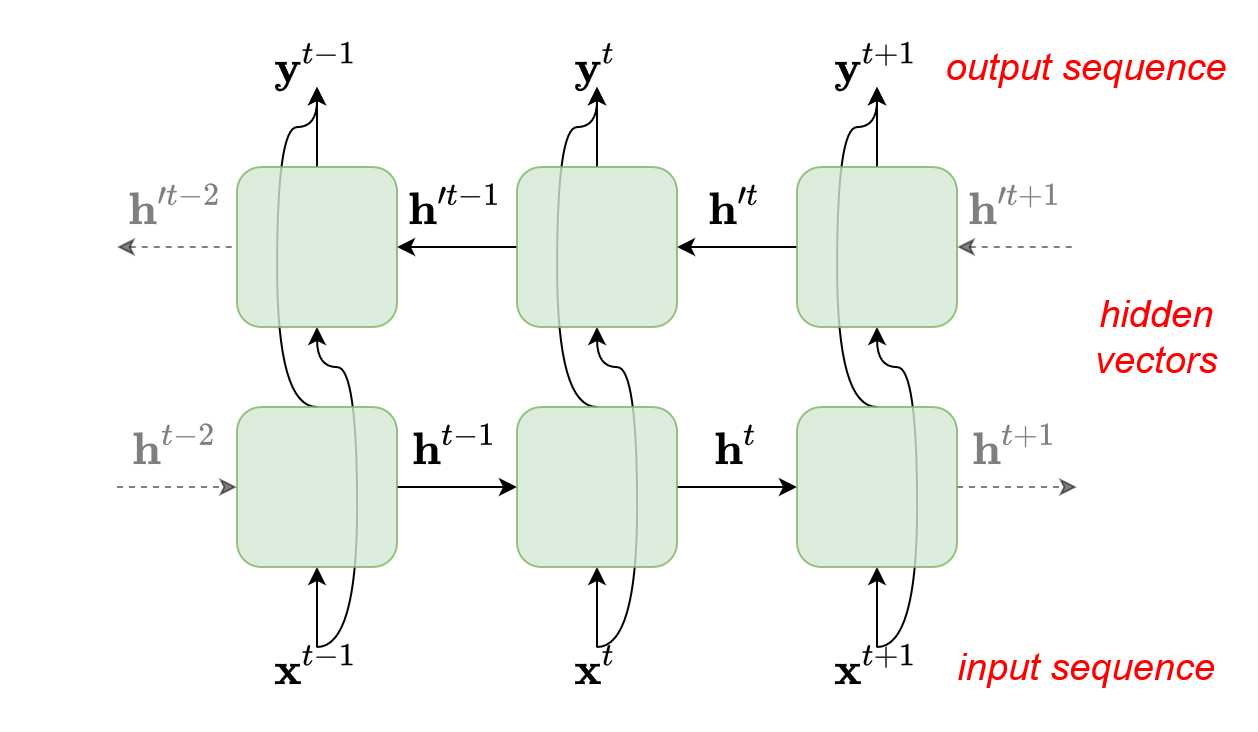
\includegraphics[width=1.\linewidth]{Images/chap3/bidirectionalRecurrentNeuralNetworks.png}
    \captionof{figure}[Bidirectional recurrent neural networks]{Bidirectional recurrent neural networks. A sequence is processed in both directions: from past to future and from future to past. This scheme can be applied for any recurrent mechanism, \textit{i.e.}, the green cells can be basic recurrent units, LSTMs or GRUs.}
    \label{fig:bidirectionalRecurrentNeuralNetworks}
    \end{center}
\end{figure}

The different types of recurrent mechanism presented above (basic recurrent layer, LSTM and GRU) are capable of processing the sequential data in a causal way. However, depending on the learning task, it could be meaningful to process the data in the other direction as well, from future to current input  (\emph{e.g.}, when looking for a music tempo, or when a whole data sequence is analyzed to obtain an overall prediction). In other words, it can be interesting to exploit information from both past and future data when processing the data at the current timestep. Bidirectional recurrent neural networks \cite{schuster_bidirectional_1997} have been introduced to address this problem. They combine recurrent layers processing the sequence from beginning to the end with recurrent layers processing the sequence the other way around. Fig~\ref{fig:bidirectionalRecurrentNeuralNetworks} illustrates how such a combination is done within the network. An input vector is fed separately into a forward layer and a backward layer, each one producing an independent output internal state vector. Thus, the next layer can benefit from two input vectors, one relying on the past and another relying on the future. Such bidirectional layers can also be applied with LSTMs or GRUs.

%-----------------------------------------------
%  RESIDUAL CONNECTIONS
%-----------------------------------------------
\section{Residual neural networks}
\label{ss:residualNetworks}

In this section we briefly present what residual neural networks consist of, and why are they useful in deep learning models.

Residual neural networks have been proposed in 2016 by He et al.~\cite{he_deep_2016} to address two common training problems encountered with very deep convolutional neural networks: the vanishing gradient problem which we presented in Section~\ref{ss:recurrentNeuralNetworks}, and the loss of accuracy resulting from the large number of layers. Their idea actually improved the performance of convolutional neural networks because it allowed for deeper architectures.

Residual neural networks are based on the desire of preserving the input features of a given layer, in addition to the output of this layer. Indeed, numerous successive transformations, applied by the multilayer structure of a deep neural network, can result in the loss of meaningful information contained in the layer's input features. By adding \textit{residual connections} between the input of a layer and its output, one can make this input feature flow through this layer unaltered (or almost, as we will see) so that it can be used further in the network.

\begin{figure}[t]
    \begin{center}
    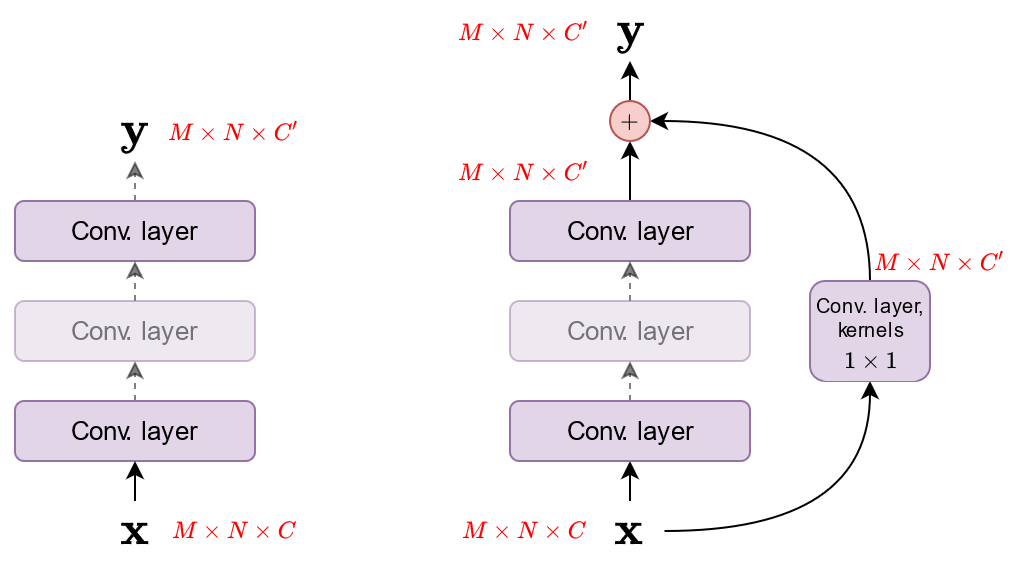
\includegraphics[width=1.\linewidth]{Images/chap3/residualBlock.png}
    \captionof{figure}[Comparison of a residual block and a classical convolutional block]{Comparison of a residual block (right) and a classical convolutional block (left). In a residual block, the input is added to the output of the last convolutional layer, eventually after its shape is adjusted using an additional convolutional layer to match the shapes.}
    \label{fig:residualBlock}
    \end{center}
\end{figure}

Fig.~\ref{fig:residualBlock} illustrates how a residual block, \emph{i.e.}, a series of layers including a residual connection, differs from a similar neural network segment without such connections. As we can see, the input of this block flows through the residual connection and is added to the output of the residual block. This residual block transforms the input using several layers, as a classical convolutional neural network usually does. However, in order to be able to add the input with the residual block output, we need to make sure to match their shapes. One trick to do this relies on inserting a convolutional layer with kernels of size $1 \times 1$ to adapt the dimensions of the input feature.

An extension of this idea has been proposed in \cite{huang_densely_2017}, where the authors propose to concatenate the input of one block with its output, instead of adding them. Their goal is to have every feature map propagated in each subsequent layer.

%-----------------------------------------------
%  ATTENTION MECHANISM
%-----------------------------------------------
\section{Attention mechanisms}
\label{sec:attentionMechanisms}


In this section we explain the attention and self-attention mechanisms. Attention models were introduced by Badhanau et al. \cite{bahdanau_neural_2015} in 2014 and refined by Luong et al. \cite{luong_effective_2015} in 2015 to improve sequence-to-sequence models. It granted neural networks with the capability to cope with long input sequences, especially in machine translation. Another great leap in natural language processing (NLP) was made with the Transformer architecture \cite{vaswani_attention_2017}, which includes the concept of \textit{self-attention}. This neural network based on an encoder-decoder scheme is very powerful to exploit the context of each word in a sentence, and has led to state-of-the-art language models such as BERT \cite{devlin_bert_2019} or GPT \cite{brown_language_2020}.

\subsection{Encoder-decoder scheme}

A sequence-to-sequence model is an architecture that takes a sequence of items (words, frames, images, etc.) as input, and process it to output another sequence of items. Such models are often constituted of two components: an encoder and a decoder. As illustrated in Fig.~\ref{fig:encoderDecoder}, an encoder is a neural network which processes the entire input sequence and computes an output vector called the \textit{context} vector. This context vector is then sent to the decoder, which is also a neural network, to output the final sequence. Before the advent of attention models, encoder and decoder were usually made of recurrent neural networks, where the context vector is actually the hidden vector of the last recurrent layer of the encoder network. The output sequence is generated item by item by the decoder, at each timestep, using the context vector to initialize its first hidden vector.

\begin{figure}[t]
    \begin{center}
    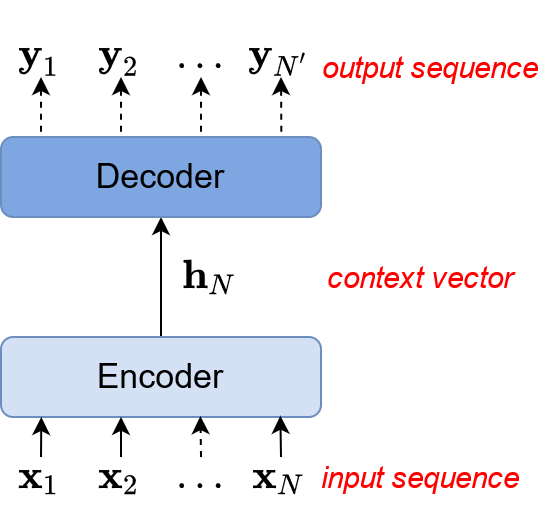
\includegraphics[width=0.5\linewidth]{Images/chap3/encoderDecoder.png}
    \captionof{figure}[Encoder-decoder scheme]{Encoder-decoder scheme. The encoder processes the entire input sequence and produces a context vector, which is then used as input for the decoder part to generate the output sequence. The input and output sequences are not necessarily of the same length.}
    \label{fig:encoderDecoder}
    \end{center}
\end{figure}


\subsection{Concept of attention}
\label{sec:attention}

As we have seen, the context vector contains all information available to the decoder to generate the output sequence. This is an issue when dealing with long input sequences, since it becomes more and more difficult to encode all relevant information from such a sequence in a single vector. Attention has been conceived to circumvent this limitation.

The first addition to the previously explained encoder-decoder scheme is that the encoder hidden vectors for all steps are passed to the decoder, instead of passing only the last hidden vector. In that way, information from each input sequence item is available to the decoder. The second novelty is the so-called attention step. The intuition is that, with regards to a particular output item, there are some items in the input sequence which are more relevant than the others. Assuming the decoder is at timestep $t$, meaning it has already output $t-1$ items, and the current hidden vector is $\mathbf{h}_{t-1}$, the attention mechanism works as follows:
\begin{itemize}
    \item a so-called \emph{attention score} is computed between all encoder hidden vectors and the current decoder hidden vector $\mathbf{h}_{t-1}$, by the means of learnable weights matrices;
    \item a softmax function is applied to all obtained attention scores so that their sum is $1$;
    \item a weighted sum of all encoder hidden vectors is calculated, using their respective softmaxed attention scores, leading to the ``current'' \textit{context} vector relevant to $\mathbf{h}_{t-1}$.
\end{itemize}
This context vector thus contains all the information about the input sequence items that is useful for the processing of the current timestep. In \cite{bahdanau_neural_2015}, the attention scores are obtained with a feedforward neural network, trained altogether with the other neural network parts. After this attention stage, the context vector is concatenated with $\mathbf{h}_{t-1}$ and is fed into another feedforward neural network, whose output is taken as the next output sequence item.

As we can see, the idea behind the attention mechanism is to provide a way for the decoding neural network to emphasize some of the input sequence items, regarding the current decoding timestep.

\subsection{Self-attention in the Transformer architecture}

The Transformer architecture is a model solely relying on the attention mechanisms, whereas previously presented models were designed as a mix of RNNs and attention. It has been proposed in 2017 by Vaswani et al. \cite{vaswani_attention_2017}, outperforming the previous models, while being more parallelizable and requiring less training time. The Transformer model is also made of encoding and decoding modules, but here each one includes several (internal) encoders and decoders, respectively. All such encoders are identical and process the input sequence items one after another.

Fig.~\ref{fig:transformerEncoder} shows the components included in one encoder. It is composed of a self-attention module, which is an attention block that compares the input sequence with itself, \emph{i.e.}, it compares each item $\mathbf{x}_i$ with the other items in the same sequence, and outputs a new corresponding vector $\mathbf{z}_i$. Then each vector $\mathbf{z}_i$ is passed independently through the same feedforward layer. The output of the encoder is therefore a new sequence of the same size as the input sequence, which can then used as the input sequence of the next encoder. 

\begin{figure}[t]
    \begin{center}
    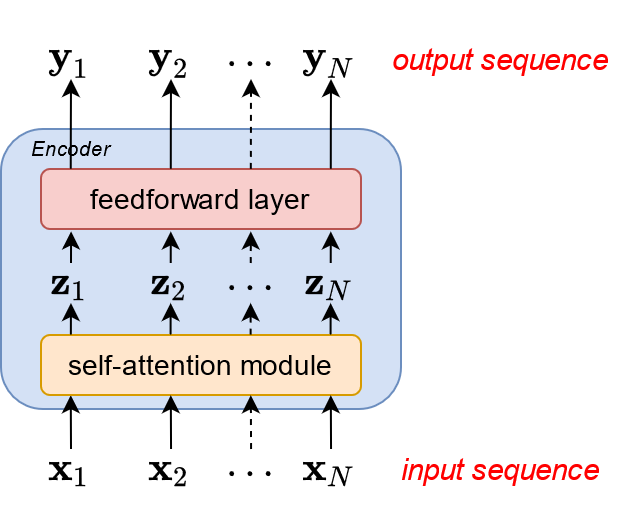
\includegraphics[width=0.6\linewidth]{Images/chap3/transformerEncoder.png}
    \captionof{figure}[Transformer's encoder components]{Transformer's encoder components. A self-attention module creates an intermediate vector $\mathbf{z}_i$ for each vector $\mathbf{x}_i$ of the input sequence. Each vector $\mathbf{z}_i$ then passed independently in a feedforward layer which produces an output sequence of the same size as the input sequence. The output sequence usually becomes the input sequence of another encoder as several encoders are stacked one after another in a typical Transformer architecture.}
    \label{fig:transformerEncoder}
    \end{center}
\end{figure}


\begin{figure}[t]
    \begin{center}
    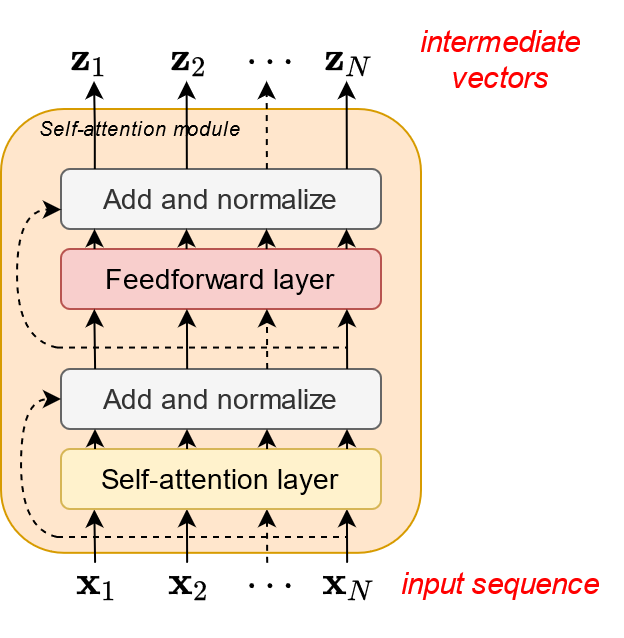
\includegraphics[width=0.6\linewidth]{Images/chap3/selfAttentionModule.png}
    \captionof{figure}[Self-attention module]{Self-attention module. In a self-attention module, the input sequence is first processed by a self-attention layer, of which the output is added to the input (using a residual connection) and the result is normalized. Then, each item of the obtained sequence goes independently through the same feedfoward layer, and the new sequence is again added to the forward layer's input sequence using a residual connection, then is normalized. Note that positional encoding, which is usually used in such encoder architecture, is not shown here as it was not used in this thesis work.}
    \label{fig:selfAttentionModule}
    \end{center}
\end{figure}

The self-attention module is illustrated in Fig.~\ref{fig:selfAttentionModule}. First, a self-attention layer actually performs the self-attention mechanism on the input sequence. For each item of the sequence $\mathbf{x}_i$, three vectors usually named \textit{query}, \textit{key}, and \textit{value} are computed. They are obtained by multiplying $\mathbf{x}_i$ with three independent weight matrices that are learnt during the training:
\begin{equation}
    \begin{aligned} 
      \mathbf{q}_i &= \mathbf{x}_i^T \mathbf{W}^Q \\
      \mathbf{k}_i &= \mathbf{x}_i^T \mathbf{W}^K. \\
      \mathbf{v}_i &= \mathbf{x}_i^T \mathbf{W}^V
    \end{aligned}
\end{equation}
Then, when encoding the item $\mathbf{x}_i$, a score $s_{ij}$ is computed with respect to every other item $\mathbf{x}_j$ as \cite{vaswani_attention_2017}:
\begin{equation}
    s_{ij} = softmax \bigg( \frac{\mathbf{q}_i \cdot \mathbf{k}_j}{\sqrt{G}} \bigg),
\end{equation}
where $G$ is the dimension of the key vectors. Finally, a new vector $\mathbf{z}_i$ is calculated as the weighted sum of the value vectors $\mathbf{v}_j$, using the computed scores as weights:
\begin{equation}
    \mathbf{z}_i = \sum_{j=1}^N s_{ij} \mathbf{v}_j,
\end{equation}
with $N$ being the sequence length. For each input sequence item $\mathbf{x}_i$ we thus obtain a new vector $\mathbf{z}_i$ that takes into account the dependencies between $\mathbf{x}_i$ and the other items (past and future) in the sequence.

The remaining components of the self-attention module shown in Fig.~\ref{fig:selfAttentionModule} are the following: a layer adds the input of the encoder to the output of the self-attention layer (sequence-wise) using a residual connection, and then normalization is applied; then each item of the obtained sequence goes independently through the same feedfoward layer, is added with the corresponding input item of this layer, with another residual connection, and is also normalized.

A last particularity for the encoder is proposed in the original paper \cite{vaswani_attention_2017}, and is called \textit{positional encoding}. The authors propose to encode the position of each input vector within the sequence using a vector $\mathbf{p}_i$ (we do not detail such encoding here, \emph{c.f.}, \cite{vaswani_attention_2017}), and append this position vector to the corresponding item $\mathbf{x}_i$, before going through the encoder.

\begin{figure}[t]
    \begin{center}
    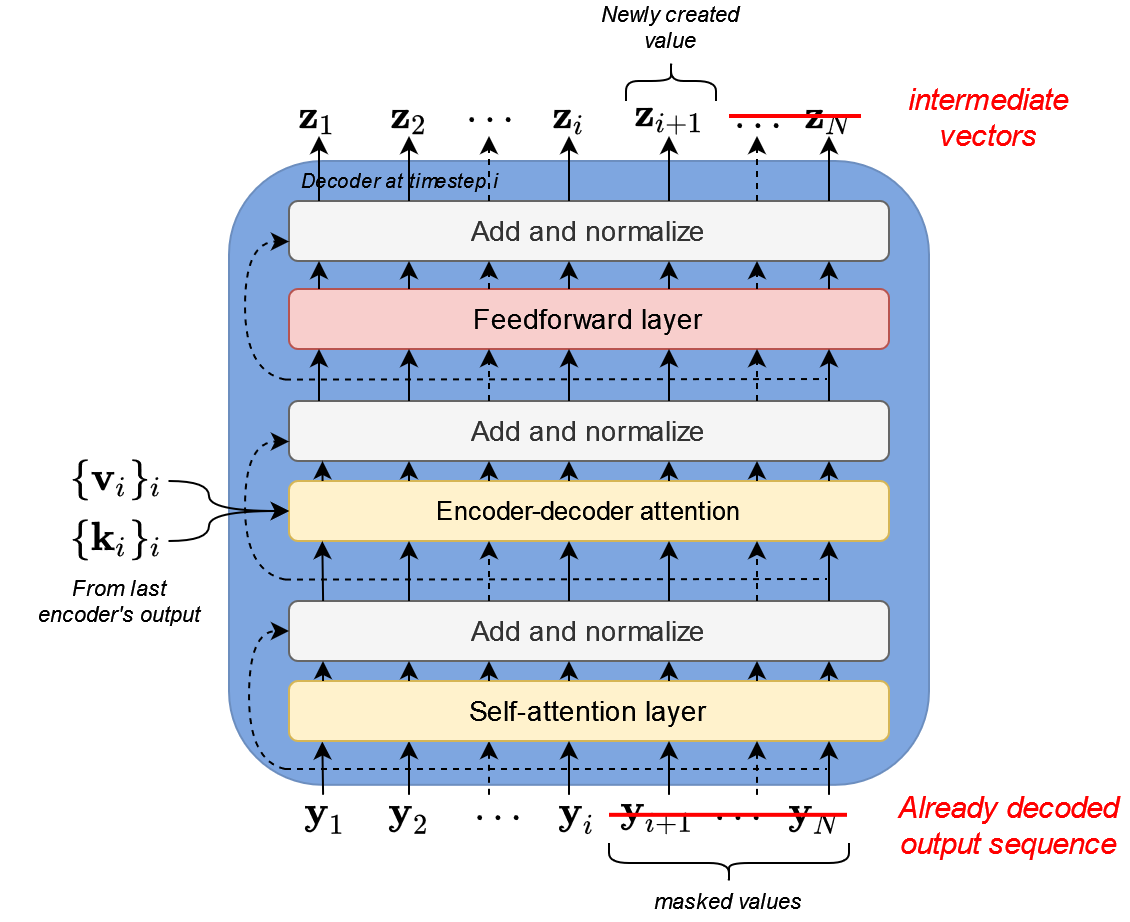
\includegraphics[width=0.85\linewidth]{Images/chap3/transformerDecoder.png}
    \captionof{figure}[Transformer's decoder module at timestep $i$]{Transformer's decoder module at timestep $i$. After a self-attention module followed by an add and normalize layer, a encoder-decoder attention module is used, and followed by another add and normalize layer. This encoder-decoder attention actually uses the key and value vectors obtained from the last encoder. Then a feedforward layer followed by an add and normalize layer is used as in en encoder module. As for the encoders, several decoders are employed and stacked one after another. As timestep $i$ (\emph{i.e.}, when decoding item $i$ of the output sequence), the previous items $1, ..., i-1$ are already decoded, and are used in the input sequence of the first decoder. The other items $i+1, ..., N$, not yet decoded, are masked in the input sequence. The newly created output item $i+1$ of the last decoder is finally used through a final layer which projects it into the target embedding space.}
    \label{fig:transformerDecoder}
    \end{center}
\end{figure}

Let us now briefly detail how the Transformer decoder part works, without going too much into details since in this thesis we only adopted the encoder in our experiments. A decoder module, illustrated in Fig.~\ref{fig:transformerDecoder}, is made of a self-attention layer, which receives the already encoded output items (the future items, not created yet, are masked during the process), followed by an add and normalize layer with residual connection. The obtained sequence is fed into another similar attention block called \textit{encoder-decoder attention} because its key and value vectors are those obtained from the output sequence of the last encoder. Finally, as in a encoder module, each obtained sequence item goes through the same feedforward layer, and then another add and normalize layer with residual connection is used. At the end, each item of the output sequence of the last decoder is projected into the target embedding space using a linear feedforward neural network, leading to the final output sequence.

\subsection{Multi-head self-attention}

In \cite{vaswani_attention_2017}, the authors actually used an extended version of the self-attention mechanism presented above. In \textit{multi-head} self-attention (MHSA), several instances of the query, key and value vectors are computed in parallel, with corresponding weights matrices $\mathbf{W}^Q$, $\mathbf{W}^K$ and $\mathbf{W}^V$. This allows a self-attention module to learn several representations for the three vectors of each item in the sequence, leading to more flexibility. When considering $H$ heads, for each item $\mathbf{x}_i$ in the input sequence we obtain $H$ vectors $\mathbf{z}_{ih}$ ($h \in [1,H]$) which are concatenated along the head dimension to give $\mathbf{\tilde{z}}_i$, and a new weight matrix $\mathbf{W}^O$ is used to obtain the final output vector $\mathbf{z}_i$:
\begin{equation}
    \mathbf{z}_i = \mathbf{\tilde{z}}_{i} \mathbf{W}^O. 
\end{equation}

In the original paper \cite{vaswani_attention_2017}, the operations to compute the self-attention scores consider the query and key vectors independently per head, \emph{i.e.}, the score for pair of item $(i,j)$ and for head $h$ is obtained by :
\begin{equation}
    s_{ijh} = \text{softmax}\Big(\frac{\mathbf{q}_{ih} \cdot \mathbf{k}_{jh}}{\sqrt{G}}\Big),
\end{equation}
where $q_{ih}$ is the query vector of item $\mathbf{x}_i$ for head $h$, and $k_{jh}$ is the key vector of item $\mathbf{x}_j$ for the same head $h$. A more general way of calculating the scores is to consider the query and key vectors across different heads $h$ and $h'$:
\begin{equation}
\label{eq:crossMultiHeadScores}
    s_{ijhh'} = \text{softmax}\Big(\frac{\mathbf{q}_{ih} \cdot \mathbf{k}_{jh'}}{\sqrt{G}}\Big).
\end{equation}
We call this more general computation \textit{cross multi-head} self-attention (CMHSA), however we did not find any literature reference considering such a mechanism. \footnote{As we will explain in a series of experiments in Sec.~\ref{chap:multisourceLocalization}, we actually performed cross-multi-head self-attention by accident while tuning our models. After investigations we understood that the scores were computed as in \eqref{eq:crossMultiHeadScores} whereas we never encountered this in the literature. We nevertheless kept these ideas since it gave interesting results} Mathematically, we can interpret a cross-multi-head mechanism with $H$ as a classical multi-head self-attention with $H^2$ heads where the query and key matrices share weights.

%-----------------------------------------------
%  CONCLUSION
%-----------------------------------------------
\section{Conclusion}
In this chapter, we provided a quick overview on different deep learning architectures that were used for designing neural models in this thesis. After presenting the basics of neuron mechanisms, we showed how feedforward neural networks, recurrent neural networks and convolutional neural networks can perform some particular tasks. We also briefly explained how residual connections work and why they are of interest. Finally, we described the basics of attention mechanism and Transformer architecture with self-attention, which are quite recent neural methods in the audio literature. Convolutional recurrent neural networks and attention mechanisms have been particularly considered in our experiments on sound source localization.
